\chapter{Estado del arte}
En este capítulo se hablará sobre el contexto en el que se enmarca este proyecto, haciendo especial mención a los paradigmas SDN y NFV.

Ambos paradigmas son la base de este Trabajo de Fin de Máster, y por ello se hace una extensa explicación de cada uno de ellos, haciendo mención a sus arquitecturas de trabajo, ya que explican de forma clara y concisa los diferentes elementos que componen dichas arquitecturas y que función desempeñan.

Una vez explicados SDN y NFV, se lleva a cabo una explicación de como han evolucionado las redes de telecomunicación en los últimos años. Esta evolución se debe a la inclusión de herramientas \textit{software}, especialmente las de código abierto, permitiendo una gestión, configuración y optimización mucho más rapida y eficiente de la infraestructura de una red de telecomunicación.

\section{SDN}
\label{sec:sdn}

SDN (\textit{Software Defined Networking})\cite{sdnbib} es un paradigma que consiste en una nueva forma de configurar y gestionar las redes de telecomunicación. Su principal premisa es la de desacoplar el plano de control y el plano de datos.

El plano de control define como se configura y gestiona la red de telecomunicación, mientras que el plano de datos es el encargado de transferir las órdenes de configuración y gestión a la infraestructura de la red.

SDN pretende cambiar la manera tradicional de configuración de dispositivos usando instrucciones de bajo nivel por una manera novedosa mediante herramientas \textit{software} a un alto nivel.

Dicho paradigma surge principalmente por las limitaciones que tienen las tecnologías de redes actualmente. Las dos principales limitaciones son:

\begin{itemize}
	\item \textbf{Dificultad de escalabilidad:} A medida que el tráfico de una red aumenta, la red debe hacer lo mismo. Esto implica nuevos dispositivos que deben ser configurados y gestionados. La cantidad de dispositivos de una red aumenta de forma exponencial, y debido a ello, la configuración y gestión tradicionales se convierte en un mecanismo tedioso y poco sostenible a largo plazo.
	
	\item \textbf{Dependencia del fabricante:} Cada fabricante diseña sus dispositivos de red de una manera particular, con su propio sistema operativo y su propia sintaxis de configuración. En una red de telecomunicaciones es habitual que su infraestructura de red esté compuesta por dispositivos de diferentes vendedores y fabricantes, y es necesario conocer a fondo cada uno de los sistemas operativos.
	
\end{itemize}

Una vez identificadas las limitaciones de redes actuales, hay que identificar los beneficios que SDN puede dar a las entidades que opten por esta tecnología en sus redes de telecomunicaciones. Los principales beneficios de SDN son:

\begin{itemize}
	\item \textbf{Reducción del CapEx (\textit{Capital Expenditures}):} CapEx son los costes asociados a bienes físicos. SDN reduce la necesidad de invertir en nuevos bienes físicos (\textit{hardware}), ya que se lleva a cabo una mejor gestión que induce a planificaciones más eficientes, con menor equipamiento se obtiene igual o menor rendimiento que de foirma tradicional.
	
	\item \textbf{Reducción del OpEx (\textit{Operational Expenditures}):} OpEx son los costes asociados a operaciones y servicios. SDN reduce este tipo de costes debido a su configuración y gestión de los elementos de red mediante \textit{software}. Este control se realiza de forma más sencilla y automática, lo que permite una reducción del tiempo empleado por los administradores de la red.
	
	\item \textbf{Agilidad y flexibilidad:} SDN permite a las diferentes entidades desplegar aplicaciones, servicios e infraestructuras de forma rápida para alcanzar objetivos en el menor tiempo posible.
\end{itemize}

\subsection{Arquitectura SDN}

Las redes definidas por \textit{software} constan de una arquitectura de red específica, compuesta por distintos componentes \textit{hardware} y \textit{software} que interactúan entre sí, como se puede ver en la figura \ref{fig:arquitecturasdn}.
 
\begin{figure}[!ht]
	\centering
	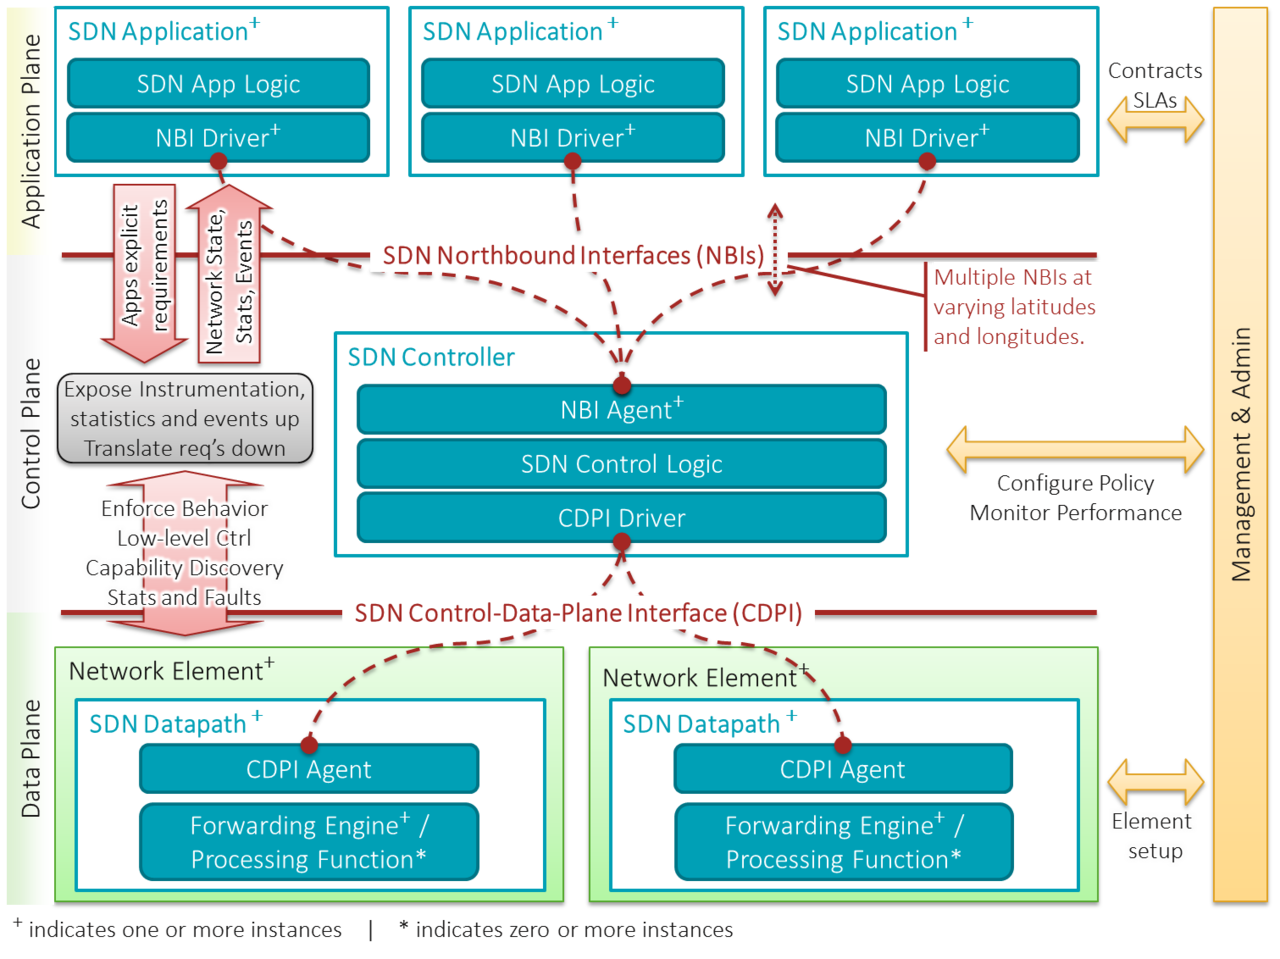
\includegraphics[width=0.75\linewidth]{imagenes/arquitectura_sdn}
	\caption{Arquitectura SDN. Fuente:\cite{sdnbib}}
	\label{fig:arquitecturasdn}
\end{figure}

Los diferentes elementos que componen la arquitectura SDN son los siguientes:

\begin{itemize}
	\item \textbf{Controlador SDN:} Es el cerebro de la red SDN. Forma el núcleo de la arquitectura SDN comunicándose con los \textit{switches} a través de la \textbf{Interfaz Sur} (\textit{SouthBound Interface}) y con las distintas aplicaciones a través de la \textbf{Interfaz Norte} (\textit{NorthBound Interface}).
	
	\item \textbf{Interfaz Sur:} Es la interfaz que conecta al controlador SDN con el plano de datos. Facilita la configuración de la red, transfiriendo dichas configuraciones a los dispositivos de la red. El protocolo más utilizado en esta interfaz es \textbf{OpenFlow} (ver \ref{subsec:openflow}).
	
	\item \textbf{Interfaz Norte:} Es la interfaz que conecta al controlador SDN con el plano de control. Facilita el proceso de automatización de la red mediante la comunicación del controlador con las diferentes aplicaciones. Para permitir dicha comunicación con las aplicaciones, la interfaz norte exporta una REST-API.
	
	\item \textbf{Agentes y \textit{Drivers}:} Para establecer la comunicación entre el controlador y los dispositivos mediante la interfaz sur y para la comunicación entre el controlador y las aplicaciones mediante la interfaz norte,es necesario un par agente-\textit{driver}. El \textit{driver} se encuentra en el controlador, mientras que el agente se encuentra en el dispositivo. Se encargan de realizar la comunicación en el plano de datos, realizando la conversión del lenguaje del controlador al del dispositivo, y viceversa.
	
	\item \textbf{Aplicaciones SDN:} Son programas que se conectan al controlador SDN mediante la interfaz norte. Gracias a su lógica de aplicaciones, desarrollan un próposito concreto y transfieren datos u órdenes al controlador SDN.
\end{itemize}


\subsection{OpenFlow}
\label{subsec:openflow}

OpenFlow\cite{openflowbib} es un protocolo estándar de SDN, siendo el más utilizado para comunicar el controlador SDN con los dispositivos que se encuentran en el plano de datos. Para que esta comunicación sea posible, el controlador SDN debe tener operando un driver OpenFlow, mientras que el dispositivo debe tener corriendo un agente OpenFlow. 

Un \textit{switch} tradicional utiliza su propia lógica de encaminamiento para decidir como tiene que reenviar los paquetes. Un \textit{switch} OpenFlow es únicamente un dispositivo \textit{hardware} que obedece órdenes que provienen del controlador SDN.

OpenFlow introduce el concepto de flujo, que sustituye a la entrada en la tabla de encaminamiento. Un flujo establece como un \textit{switch} OpenFlow procesa un paquete determinado. Un flujo se compone de dos partes:

\begin{itemize}
	\item \textbf{Selector o regla:} El selector define el conjunto de reglas que debe seguir un determinado paquete. Por ejemplo: tener una dirección MAC origen y/o destino específicas, o una dirección IP origen y/o destino específicas. 
	
	\item \textbf{Tratamiento o acción:} El tratamiento define como se va a procesar un determinado paquete. Por ejemplo: ser reenvíado por un determinado puerto o ser enviado directamente al controlador SDN.
\end{itemize}
	
A continuación, se empieza ya a hablar más en detalle de un \textit{switch} OpenFlow. Dicho componente tiene las siguientes partes:

\begin{itemize}
	\item \textbf{Agente o Cliente OpenFlow:} Es el encargado de comunicarse con el driver OpenFlow que se encuentra en el controlador SDN.
	
	\item \textbf{Tabla de flujos:} Es la tabla donde se almacenan los flujos del \textit{switch}. Mantiene una relación entre el selector y el tratamiento, así como diferentes estadísticas de monitorización.
	
	\item \textbf{Puerto:} Este concepto es similar al de un \textit{switch} tradicional.
\end{itemize}

\section{NFV}
\label{sec:nfv}

NFV (\textit{Network Function Virtualization})\cite{nfvbib} es un paradigma que engloba a las redes de telecomunicación, más concretamente a su infraestructura. Su principal premisa es la de desacoplar las funciones de red de dispositivos \textit{hardware} y trasladarlas a servidores virtuales. Con ello se consigue tener múltiples funciones virtualizadas en un único servidor.

Las redes de telecomunicación actuales tienen ciertos problemas que NFV pretende resolver, como son:

\begin{itemize}
	\item Altos costes y restricciones físicas de fabricación.
	\item Complejidad \textit{hardware} en las soluciones del fabricante.
	\item Ciclo de vida corto de los dispositivos \textit{hardware}.
\end{itemize}

Todos estos problemas o desventajas han desembocado en la adopción de NFV como un estándar para agilizar, facilitar y escalar las infraestructuras de red, así como disminuir costes.

NFV tiene una serie de ventajas importantes que lo convierte en un alternativa óptima:

\begin{itemize}
	\item \textbf{Simplificar la implantación de elementos de red:} Las soluciones de red NFV son flexibles, genéricas y fáciles de implantar, lo que implica que el proceso de actualización es también más rápido y sencillo.
	
	\item \textbf{Mayor escalabilidad de la red:} Gracias a la naturaleza \textit{software} de las funciones virtualizadas, es mucho más fácil escalar los componentes de la red que si se trataran de dispositivos físicos.
	
	\item \textbf{Independencia respecto a los fabricantes de dispositivos:} Debido a que las funciones virtualizadas son desarrolladas mediante \textit{software}, se pierde la dependencia respecto a las particularidades de cada dispositivo, como su sistema operativo o su sintáxis de configuración y gestión, entre otros.
\end{itemize}

\subsection{Arquitectura NFV}
\label{subsec:nfvarq}

La virtualización de funciones de red consta de una arquitectura específica, compuesta por diferentes componentes \textit{hardware} y \textit{software} que interactúan entre sí, como se puede ver en la figura \ref{fig:arquitecturanfv}.

\begin{figure}[!ht]
	\centering
	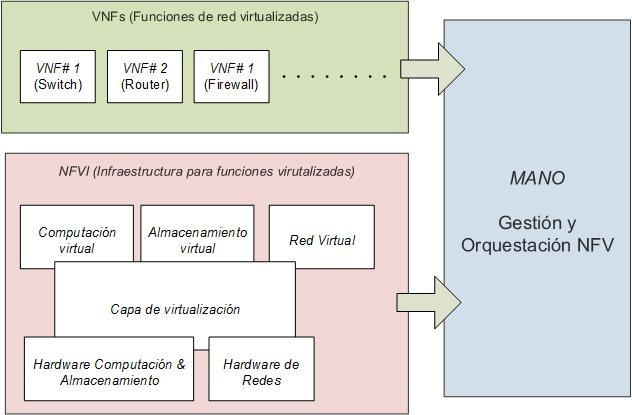
\includegraphics[width=0.75\linewidth]{imagenes/arquitectura_nfv}
	\caption{Arquitectura NFV}
	\label{fig:arquitecturanfv}
\end{figure}

La arquitectura NFV se compone principalmente de tres componentes, descritos a continuación:

\begin{itemize}
	\item \textbf{Infraestructura NFV:} Es el componente que constituye la base de la arquitectura. Se trata del conjunto de equipos \textit{hardware} y sus recursos (CPU, RAM, HD entre otros) que se utilizan para alojar las máquinas virtuales que componen las diferentes funciones de red virtualizadas (VNFs).
	
	\item \textbf{Bloque de VNFs:} Es el componente que engloba al conjunto de VNFs disponibles para instanciar. Una VNF viene descrita como un conjunto de máquinas virtuales que utilizan determinados recursos de la infraestructura.
	
	\item \textbf{MANO (\textit{Manager and Orchestrator}):} Es el componente que interactúa tanto con la infraestructura NFV como con el bloque de VNFs. Se encarga de gestionar y orquestar a la propia infraestructura, controlando las acciones que sobre ella se realizan. Dichas acciones pueden ser una nueva instanciación de una VNF o un borrado de una VNF existente, entre otras.
	
\end{itemize}

Después de haber explicado cada uno de los tres componentes de la arquitectura NFV, es necesario poner un ejemplo completo de como se instancia una nueva función de red virtualizada, explicando las interacciones entre los componentes:

\begin{enumerate}
	\item El usuario elige una VNF del bloque de VNFs para instanciar. Dicha orden es transferida al bloque MANO.
	\item El bloque MANO solicita a la infraestructura NFV información sobre sus recursos disponibles, para comprobar si la VNF podrá ser instanciada o no.
	\item En caso afirmativo, el bloque MANO recibirá un OK de la infraestructura y procederá a mandar la orden de instanciación.
	\item Una vez enviada la orden de instanciación, la infraestructura NFV reservará los recursos necesarios y arrancará el conjunto de máquinas virtuales pertenecientes a la VNF instanciada.
	\item Si la instanciación ha sido correcta, el bloque MANO recibirá un OK, que será retransmitido al usuario.
	\item El bloque MANO, gracias a su interacción con la infaestructura NFV, proveerá al usuario de datos de monitorización de la VNF instanciada.
\end{enumerate}

\section{Relación entre SDN y NFV}
\label{sec:sdnnfv}

SDN es un conjunto de técnicas para agilizar la gestión y configuración de redes de telecomunicación gracias a herramientas \textit{software}. En cambio, NFV es un paradigma que persigue un cambio total en la infraestructura de una red de telecomunicación mediante el uso de funciones de red virtualizadas que sustituyan a los dispositivos físicos.

Puede parecer que ambas tecnologías tienen objetivos totalmente diferentes, pero gracias a su uso conjunto, ambos objetivos han convergido a uno solo, el de crear el concepto de NSC (\textit{Network Service Chaining}).

NSC utiliza técnicas SDN y NFV para definir el concepto de \textit{Service Chain}, una cadena de servicio. Ésta viene definida por un origen y un destino, y por un conjunto de servicios de red que deben ser atravesados en un orden específico.

\begin{figure}[!ht]
	\centering
	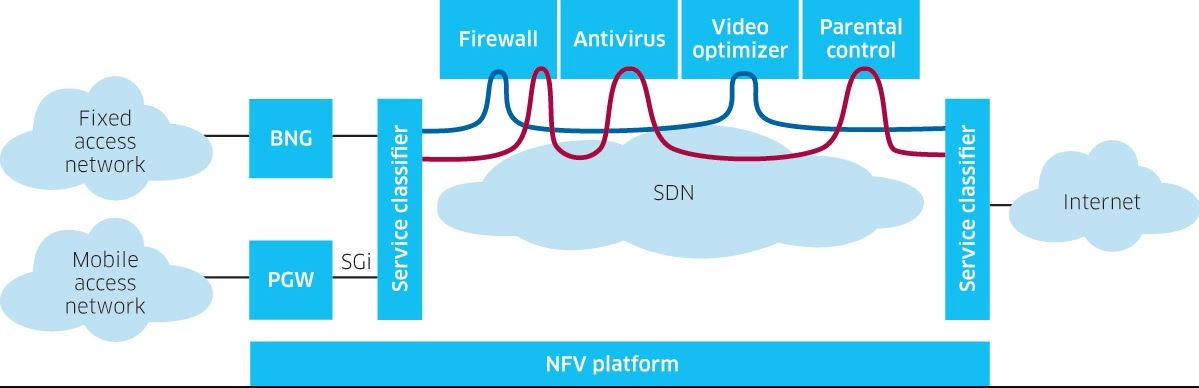
\includegraphics[width=0.8\linewidth]{imagenes/servicechaining}
	\caption{Ejemplo de \textit{Service Chaining}}
	\label{fig:servicechaining}
\end{figure}

En la figura \ref{fig:servicechaining} se puede observar como está constituida una \textit{Service Chain}. Existen un origen y un destino, y un conjunto de servicios de red (Firewall, Antivirus, Optimizador de vídeo y Control Parental)


\section{Herramientas Open-Source en redes de telecomunicación}
\label{sec:opensourcenets}

Una red de telecomunicación es un conjunto de medios, tecnologías y protocolos que tienen como finalidad el intercambio de información entre diferentes usuarios.

Así mismo, se está produciendo una enorme evolución en el concepto de una red de telecomunicación. 

En los orígenes, este concepto era puramente físico, con un conjunto de dispositivos \textit{Hardware}, como pueden ser \textit{routers}, \textit{switches} u ordenadores, interactuando entre sí. Actualmente, la gran mayoría de las redes de telecomunicación utilizan software open-source para diferentes propósitos:

\begin{itemize}
	\item Sacar el máximo rendimiento a su infraestructura.
	\item Agilizar el envío y procesamiento del tráfico de la red.
	\item Acelerar y automatizar la gestión y configuración de los dispositivos.
	\item Reducir los costes de operación de la red.
\end{itemize}

Para conseguir los propósitos mencionados anteriormente, existen numerosas herramientas de software desarrolladas por empresas, universidades u organizaciones que están totalmente disponibles para ser usadas por cualquier usuario.

Dichas herramientas forman un gran conjunto heterogéneo, siendo desarrollada cada una de ellas para uno o más propósitos:

\begin{itemize}
	\item Para sacar el máximo rendimiento a la infraestructura de una red, existen herramientas de virtualización como \textbf{OpenStack} (ver \ref{sec:openstack}) o \textbf{Docker}, para proveer a las aplicaciones de una abstracción e independencia. Este tipo de herramientas se enmarcan dentro de la tecnología \textbf{NFV} (ver \ref{sec:nfv}).
	
	\item Para agilizar el envío y procesamiento del tráfico de una red, existen herramientas que permiten emular el comportamiento de diversos dispositivos hardware a través de la virtualización, como \textbf{OpenVSwitch} o \textbf{Mininet} (ver \ref{sec:mininet}). Gracias a este tipo de herramientas, se puede sustituir un \textit{Switch} clásico por un pequeño software que hace las funciones de un \textit{Switch} de una manera más eficiente.
	
	\item La gestión de los dispositivos se ha realizado de forma manual, dispositivo a dispositivo. Gracias a herramientas software como \textbf{Cacti} o \textbf{Nagios}, la forma de gestionar las redes de telecomunicación ha dado un giro de 180 grados. Utilizando estas herramientas, el usuario puede gestionar la red desde un terminal de manera remota, gracias al protocolo SNMP (\textbf{Simple Network Management Protocol}).
	
	\item Para acelerar y automatizar la configuración de los dispositivos de una red de telecomunicación, existen herramientas enmarcadas en la tecnología \textit{SDN} (ver \ref{sec:sdn}). Un ejemplo de estas herramientas es el controlador SDN ONOS (ver \ref{sec:onos}).
	
	\item Para reducir los costes de operación de una red, existen herramientas open-source que ayudan a planificar una red de telecomunicación de forma óptima. La más conocida de estas herramientas es \textbf{Net2Plan} (ver \ref{sec:net2plan}), una herramienta de planificación de redes programada en Java.
\end{itemize}



\cleardoublepage